%%%%%%%%%%%%%%%%%%%%%%%%%%%%%%%%%%%%%%%%%
% Journal Article
% LaTeX Template
% Version 2.0 (February 7, 2023)
%
% This template originates from:
% https://www.LaTeXTemplates.com
%
% Author:
% Vel (vel@latextemplates.com)
%
% License:
% CC BY-NC-SA 4.0 (https://creativecommons.org/licenses/by-nc-sa/4.0/)
%
% NOTE: The bibliography needs to be compiled using the biber engine.
%
%%%%%%%%%%%%%%%%%%%%%%%%%%%%%%%%%%%%%%%%%

%----------------------------------------------------------------------------------------
%	PACKAGES AND OTHER DOCUMENT CONFIGURATIONS
%----------------------------------------------------------------------------------------

\documentclass[
	a4paper, % Paper size, use either a4paper or letterpaper
	10pt, % Default font size, can also use 11pt or 12pt, although this is not recommended
	unnumberedsections, % Comment to enable section numbering
	twoside, % Two side traditional mode where headers and footers change between odd and even pages, comment this option to make them fixed
]{LTJournalArticle}
\usepackage{biblatex}
\usepackage{authblk} 
\usepackage{caption}
\captionsetup{width=.5\textwidth}
\addbibresource{biblio.bib} % BibLaTeX bibliography file

\runninghead{ANLP project report} % A shortened article title to appear in the running head, leave this command empty for no running head

\footertext{\textit{ANLP} (2025) Kaggle Project} % Text to appear in the footer, leave this command empty for no footer text

\setcounter{page}{1} % The page number of the first page, set this to a higher number if the article is to be part of an issue or larger work

%----------------------------------------------------------------------------------------
%	TITLE SECTION
%----------------------------------------------------------------------------------------

\title{ANLP Kaggle project\\ \LARGE Language identification (LID)} % Article title with subtitle


% Authors are listed in a comma-separated list with superscript numbers indicating affiliations
% \thanks{} is used for any text that should be placed in a footnote on the first page, such as the corresponding author's email, journal acceptance dates, a copyright/license notice, keywords, etc
\author{%
    Ilann Amiaud--Plachy\textsuperscript{1},
    Thomas Bodart\textsuperscript{1},
    Maceo Duriez\textsuperscript{1},
    Marc-César Garcia-Grenet\textsuperscript{1},
    Gaétan Jacquemin\textsuperscript{1}
}

\date{\footnotesize\textsuperscript{\textbf{1}}CentraleSupélec, Paris-Saclay University}

% Affiliations are output in the \date{} command
% \date{\footnotesize\textsuperscript{\textbf{1}}Immersive Audio, L-Acoustics UK Ltd\\ \textsuperscript{\textbf{2}}MSc Student in Information and Comms. Eng., CentraleSupélec, Paris-Saclay University}

% Full-width abstract
\renewcommand{\maketitlehookd}{%
	\begin{abstract}
		L’identification de langue (LID) est une tâche essentielle en traitement du langage naturel (NLP), jouant un rôle clé dans de nombreuses applications multilingues. Dans le cadre du projet Kaggle du cours d’ANLP, nous avons exploré différentes approches, à la fois statistiques et basées sur l’apprentissage profond, afin de développer un modèle performant de LID. Après comparaison, notre solution finale combine FastText, rapide et efficace pour la classification de texte, avec roBERTa, un modèle transformer offrant une meilleure capacité de généralisation, en utilisant les probabilités données par les modèles.
	\end{abstract}
}

%----------------------------------------------------------------------------------------
%----------------------------------------------------------------------------------------

\begin{document}
\maketitle % Output the title section

%----------------------------------------------------------------------------------------
%	ARTICLE CONTENTS
%----------------------------------------------------------------------------------------

\section{Introduction}

    
La détection automatique de la langue représente un fort enjeux pour diverse application, en premier lieu pour la traduction mais surtout pour l'organisation automatique de contenus multilingues, très utile pour la collecte de données à grand échelle. Permettant de rassembler des corpus plus gros et plus précis utilisés pour entraîner des modèles qui requièrent toujours plus de data.

Les approchent traditionnelles historiques de détection linguistique sont surtout des approches statistiques comme les n-grammes \cite{cavnar1994n} ou TF-IDF \cite{baldwin2010language}. Mais aujourd'hui il est pertinent d'évaluer la performance des modèles de language neuronaux pré-entrainésur des grands corpus multilingues comme BERT \cite{devlin2019bert}.

Dans notre étude, nous avons exploré et comparé plusieurs approches :
\begin{itemize}
    \item Une approche classique utilisant TF-IDF avec un classificateur SVM
    \item FastText, qui exploite efficacement les représentations de sous-mots \cite{joulin2017bag}
    \item Des modèles transformers multilingues comme mBERT \cite{devlin2019bert} et XLM-RoBERTa \cite{conneau2020unsupervised}
\end{itemize}

Nos expérimentations ont révélé que [MODÈLE] obtient les meilleures performances avec une précision de [SCORE]\%. Ce résultat peut s'expliquer par [RAISON]. Cependant, nous avons également observé que [OBSERVATION INTÉRESSANTE] concernant [ASPECT SPÉCIFIQUE].

La suite de ce rapport est organisée comme suit : la section 2 présente plus précisémenent les solutions que nous avons essayés, et la section 3 présente et discute des résultats.



\section{Solutions}

    \subsection{Exploration du dataset et preprocessing}

Le fichier d'entraînement train\_submissions.csv proposé pour cette compétition kaggle est un fichier csv de 3 colonnes Usage, Text, Label et 190599 lignes avec 389 labels cibles. Parmi ces 190599 lignes, 500 d'entre elles ne possèdent pas de label. 

On peut noter que les labels sont déséquilibrés, comme le montre la figure suivante :

\begin{figure}[h!]
    \centering
    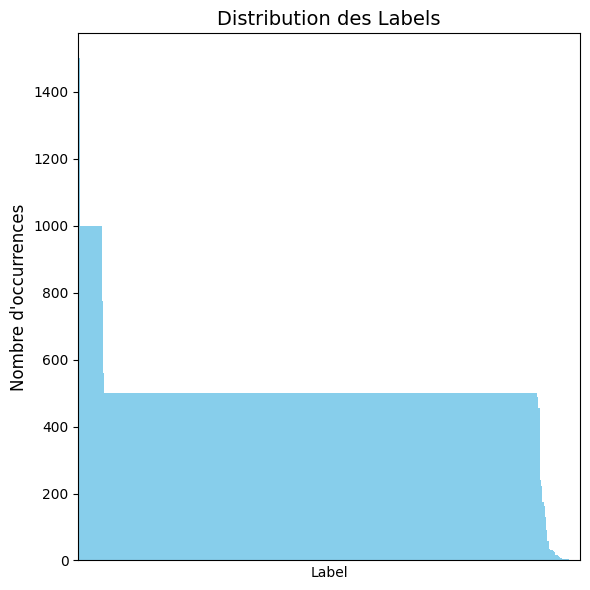
\includegraphics[width=0.5\textwidth, height=7cm]{img/unbalance.png}
    \caption{Distribution déséquilibrée des labels dans le dataset}
    \label{fig:unbalance}
\end{figure}

Nous avons essayé plusieurs techniques de downsampling et d'oversampling pour palier au déséquilibre des données, notamment en essayant d'enrichir les labels avec le moins de données disponibles grâce à des LLMs. Néanmoins cette approche n'a pas donné de bon résultats car cela retirait une partie des biais inhérents au dataset. Nous avons donc fait le choix de downsampler les labels ayant plus de 500 labels en choisissant 500 lignes aléatoirement parmi ces labels.

Il est à noté que le dataset comprenait de nombreuses langues régionales très peu parlées donc males prises en charge par de nombreux modèles pré-entrainé. De plus, pour ces langues la quantité de données pour l'entrainement était assez faible puisque plus de 50\% des textes ne comportaient pas plus de 16 mots. 

Enfin nous pouvons également souligné la présence de nombreuses langues très répandues telles que l'anglais, l'espagnol ou encore le français qui représentait parfois la totalité de certains textes pourtant labellisé dans une autre langue. C'est pourquoi lors de nos différentes tentatives le recall obtenu sur ces différentes langues s'avérait plus faible comparativement à des langues moins usitées.

Pour ce qui est du preprocessing, nous avons décidé d'appliquer un preprocessing assez simple en retirant notamment les chaînes de caractères n'apportant pas d'informations sur la langue tels que les emojis ou les adresses mails.

\subsection{TF-IDF}

TF-IDF est une méthode statistique utilisée pour évaluer l'importance d'un mot dans un document par rapport à une collection de documents. Elle combine deux métriques : la fréquence du terme (TF) et la fréquence inverse du document (IDF). La fréquence du terme mesure combien de fois un mot apparaît dans un document, tandis que l'IDF diminue l'importance des mots qui apparaissent fréquemment dans tous les documents.

Pour notre utilisation, TF-IDF nous permet de créer des vecteurs de représentation à partir des textes, puis d'entraîner un classifieur pour évaluer la langue du texte. Dans notre cas, nous avons utilisé un classifieur SVM car c'est celui qui, théoriquement et expérimentalement, donne les meilleurs résultats (voir \cite{baldwin2010language}).

Cette approche nous a donné des résultats assez satisfaisants mais pas suffisants pour notre cas d'utilisation et s'est laissé largement dépasser par les autres approches, certainement car elle ne prend pas en compte les relations entre les mots et les contextes dans lesquels ils apparaissent.

\subsection{FastText}

FastText est une bibliothèque développée par Facebook \cite{joulin2017bag} pour la représentation de mots et l'apprentissage de classificateurs de texte. Comme vu en cours, elle repose sur des modèles de type n-grammes pour capturer des informations sur les sous-mots, ce qui permet de mieux gérer les mots rares et les fautes d'orthographe.

FastText est particulièrement efficace pour l'identification de langue car il peut capturer des caractéristiques spécifiques à chaque langue au niveau des sous-mots. Il a donné de très bons résultats dans notre étude, avec des scores similaires voire supérieurs aux modèles de langage neuronaux (voir ci-dessous), mais avec des temps d'entraînement et d'inférence presque instantanés en comparaison.

Pour son entraînement, nous avons dans un premier temps pris les hyperparamètres donnés dans l'article GlotLID \cite{Kargaran_2023}, un article présentant un modèle classifiant plus de 1800 langues, puis nous avons fait une recherche d'hyperparamètres aux alentours de ces derniers. 

\begin{table}[h]
    \centering
    \small
    \begin{tabular}{lcc}
        \hline
        \textbf{Argument} & \textbf{Description} & \textbf{Valeur} \\
        \hline
        -minCount & Occurrences min mot & 1000 \\
        -minCountLabel & Occurrences min label & 0 \\
        -wordNgrams & Max n-grammes mots & 1 \\
        -bucket & Nb de buckets & $10^6$ \\
        -minn & Min. n-gram caractères & 1 \\
        -maxn & Max. n-gram caractères & 5 \\
        -loss & Perte & softmax \\
        -dim & Taille vecteurs & 256 \\
        -epoch & Nombre d'époques & 9 \\
        -lr & Taux apprentissage & 1.5 \\
        \hline
    \end{tabular}
    \caption{Hyperparamètres d'entraînement du modèle FastText}
    \label{tab:glotlid-m-hyperparams}
\end{table}

\subsection{mBERT}

mBERT (Multilingual BERT) est la version multilingue du modèle BERT \cite{devlin2019bert}, qui est un modèle de langage basé sur des transformers, possédant 179M de paramètres. Sa particularité est qu'il est pré-entraîné sur la tâche de Masked Language Model, sur un vaste corpus de textes dans 104 langues, ce qui lui permet de comprendre et de générer des représentations contextuelles pour des textes dans différentes langues.

Ce modèle fut notre première approche de langage neuronal pour ce projet.  Nous avons de même utilisé le tokenizer correspondant à mBERT, comprenant tous les caractères de notre corpus, et nous n'avons pas mis de limite de taille pour le nombre de tokens. Nous avons d'abord essayé une méthode de transfert (transfer learning) pour adapter mBERT à notre tâche, mais cela s'est avéré insuffisant et il a finalement fallu ajuster les poids du modèle (fine-tuning) pour obtenir des résultats satisfaisants sur 10 epochs, en utilisant 85\% du dataset fourni en train, et une dernière epoch en utilisant la totalité du corpus, pour utiliser le plein potentiel de nos données. L'inconvénient de cette méthode est qu'elle est très lourde en calculs (plusieurs heures d'entraînement).

Finalement, mBERT a donné des résultats satisfaisants mais s'est logiquement laissé dépasser par XLM-RoBERTa (voir ci-dessous), qui possède en particulier plus de paramètres.

\subsection{XLM-RoBERTa}

XLM-RoBERTa \cite{conneau2020unsupervised} est une variante optimisée de BERT \cite{devlin2019bert} qui utilise un processus d'entraînement plus robuste et une plus grande quantité de données sur 100 langues. Nous avons utilisé le modèle base à 279M de paramètres. Les améliorations incluent l'entraînement sur des lots de données plus grands, l'utilisation de plus de données d'entraînement, et l'optimisation des hyperparamètres. C'est donc très logiquement que nos résultats suivent l'amélioration promise par les chercheurs à son origine et qu'il surpasse mBERT.

Notre utilisation reprend la même logique que pour mBERT avec une nette amélioration des performances, mais avec un coût en temps d'entraînement et d'inférence plus élevé. Pour palier à cela, nous avons décidé de restreindre chaque phrase à 128 tokens, avec un padding si la phrase contient moins de 128 tokens, et un troncage si elle en contient plus. Cela a drastiquement réduit le temps d'entraînement. Nous avons également utilisé un taux d'apprentissage de 2e-5, un batch size de 64, et un nombre d'époques de 10. On a de plus utilisé le tokenizer de XLM-RoBERTa.

\subsection{Combinaison FastText et XLM-RoBERTa}

Il nous est naturellement venu l'envie de combiner nos modèles portant sur des approches différentes pour tenter de profiter des avantages de chaques approches, pour améliorer les performances de notre solution. La combinaison qui nous a donné les meilleurs résultats après divers essais est la suivante : si l'inférence avec FastText donne une prédiction avec une probabilité supérieure à 0.99\%, on la garde ; sinon, on utilise XLM-RoBERTa pour donner une prédiction. Nous avons fait une étude de sensibilité sur le seuil de probabilité de FastText, et 0.99\% est le seuil qui nous a donné les meilleurs résultats, et, en effet, les prédictions au dessus de ce seuil ont une accuracy de 99\% sur le val.

\section{Resultats et Analyses}

    

Pour évaluer la performance de nos modèles, nous utilisons l'accuracy comme métrique principale. Cette métrique est particulièrement pertinente dans notre cas, car les classes sont relativement équilibrées dans notre corpus, y compris dans l'ensemble de test.

Les résultats obtenus pour les différents modèles sont présentés dans le tableau~\ref{tab:results}.

\begin{table}[ht]
    \centering
    \begin{tabular}{lcccc}
        \toprule
        Modèle & Val acc & Test acc  & inférence* \\
        \midrule
        FastText & 0.86 & 0.84 & 63s \\
        TFIDF & 0.34 & 0.33 & 30s \\
        mBERT & 0.86 & 0.86 & 1h15 \\
        XLM-roBERTa & 0.87 & 0.87 & 1h \\
        FT + XLM-R & 0.88 & 0.88 & 1h \\
        \bottomrule
    \end{tabular}

    \caption{Accuracy sur le val et sur le test des modèles essayés. (*durée d'inférence sur un ordinateur classique avec GPU sur tout le corpus de texte)}
    
    \label{tab:results}
\end{table}
\subsection{Performance globale des modèles}

Comme attendu, les modèles neuronaux de grande taille (mBERT, XLM-RoBERTa) offrent des performances élevées, avec une accuracy test atteignant 0.86 et 0.87 respectivement. Ces résultats confirment que les modèles de type Transformer sont particulièrement efficaces pour la tâche de détection de langues, grâce à leur capacité à capturer des représentations riches et contextuelles des textes.

Toutefois, cette performance a un coût : le temps d'inférence est particulièrement élevé. Par exemple, mBERT nécessite \textbf{1h15} pour traiter l'ensemble du corpus, ce qui peut poser des contraintes importantes dans un contexte de production ou de traitement en temps réel.

Le modèle TF-IDF, basé sur une approche purement statistique, affiche des résultats bien inférieurs (\textbf{0.34 d’accuracy}), ce qui montre ses limites face aux approches basées sur l’apprentissage automatique. Cela est sûrement dû à la présence de dialectes très proches.

\subsection{L'exception FastText}

Un résultat particulièrement intéressant est celui de \textbf{FastText}, qui atteint \textbf{0.84 d'accuracy en test}, soit un score très proche de ceux obtenus avec des modèles neuronaux beaucoup plus lourds. Ce modèle présente un énorme avantage : son \textbf{temps d'inférence est quasi instantané} (1 min sur l’ensemble du corpus de 200K instances). Cela en fait un candidat idéal pour des applications nécessitant un traitement rapide et efficace, comme la classification de textes en temps réel ou l’analyse de grandes quantités de données avec des ressources limitées.

\subsection{Vers une combinaison optimale : FT + XLM-R}

Face à ces observations, nous avons cherché à combiner les forces de nos différents modèles pour accroître l'accuracy et être plus performant sur le concours. L’association de \textbf{FastText et XLM-RoBERTa} (FT + XLM-R) a permis d’atteindre une \textbf{accuracy de 0.88}, soit la meilleure performance obtenue parmi tous les modèles testés.
En combinant ces deux modèles, nous obtenons un système performant qui optimise le \textbf{l'accuracy} bien qu'elle ne permette pas de réduire le temps d'inférence.

\section{Conclusion et perspectives}

Nos résultats montrent que, bien que les modèles de type Transformer offrent d’excellentes performances en détection de langues, leur coût en calcul reste un défi majeur. FastText s’est révélé être une alternative étonnamment efficace, capable d’obtenir des résultats proches des modèles neuronaux tout en étant extrêmement rapide.

La combinaison de FastText avec XLM-RoBERTa permet de tirer parti des avantages des deux approches, offrant ainsi une solution optimisée pour la détection de langues à grande échelle. Dans le futur, des recherches pourraient être menées pour affiner davantage le temps d'inférence de notre meilleur modèle tout en conservant son excellente précision, notamment en explorant des techniques comme la \textbf{distillation de connaissances}, où un modèle léger apprend à reproduire les décisions d’un modèle plus complexe. 
Pour aller plus loin au niveau de la précision, il serait intéressant d'explorer plus en profondeur, et avec plus de temps les hyperparamètres de nos grands modèles de langages neuronaux, pour voir si nous pouvons encore améliorer les performances, voir de tester, avec une puissance de calcul plus importante, des modèles plus grands comme RoBERTa large, possèdant 355M de paramètres.




    \printbibliography


\end{document}
